\documentclass[11pt]{amsart}
\usepackage{geometry}                % See geometry.pdf to learn the layout options. There are lots.
\geometry{a4paper}                   % ... or a4paper or a5paper or ... 
%\geometry{landscape}                % Activate for for rotated page geometry
\usepackage[parfill]{parskip}    % Activate to begin paragraphs with an empty line rather than an indent
\usepackage{graphicx}
\usepackage{amssymb}
\usepackage{amsmath}
\usepackage{epstopdf}
\DeclareGraphicsRule{.tif}{png}{.png}{`convert #1 `dirname #1`/`basename #1 .tif`.png}
\usepackage[utf8]{inputenc}
\usepackage[ngerman]{babel}
\usepackage{placeins}

\title{\(\boldsymbol{8^3}\) LED Würfel}
%\title{8x8x8 LED Würfel}
\author{Felix Bäder, Thomas Buck, Max Nuding}
\date{}                                           % Activate to display a given date or no date

\begin{document}
\maketitle

% ###############################

\section{Überblick}

Ein LED Würfel aus 512 LEDs und mit einer Kantenlänge von 8 LEDs wird von einem AVR Prozessor gesteuert. Mittels einer PC-Software können Animationen für den Würfel erstellt und in dessen Speicher geladen werden.

Alternativ können die Amplituden eines Audio Signals von einem weiteren Prozessor ausgewertet werden, um diese auf dem LED Würfel zu visualisieren.

% ###############################

\section{Hardware - AtMega32}
\begin{figure}[hbp]
	\begin{minipage}[t]{6cm}
		\vspace{0pt}
		\centering
		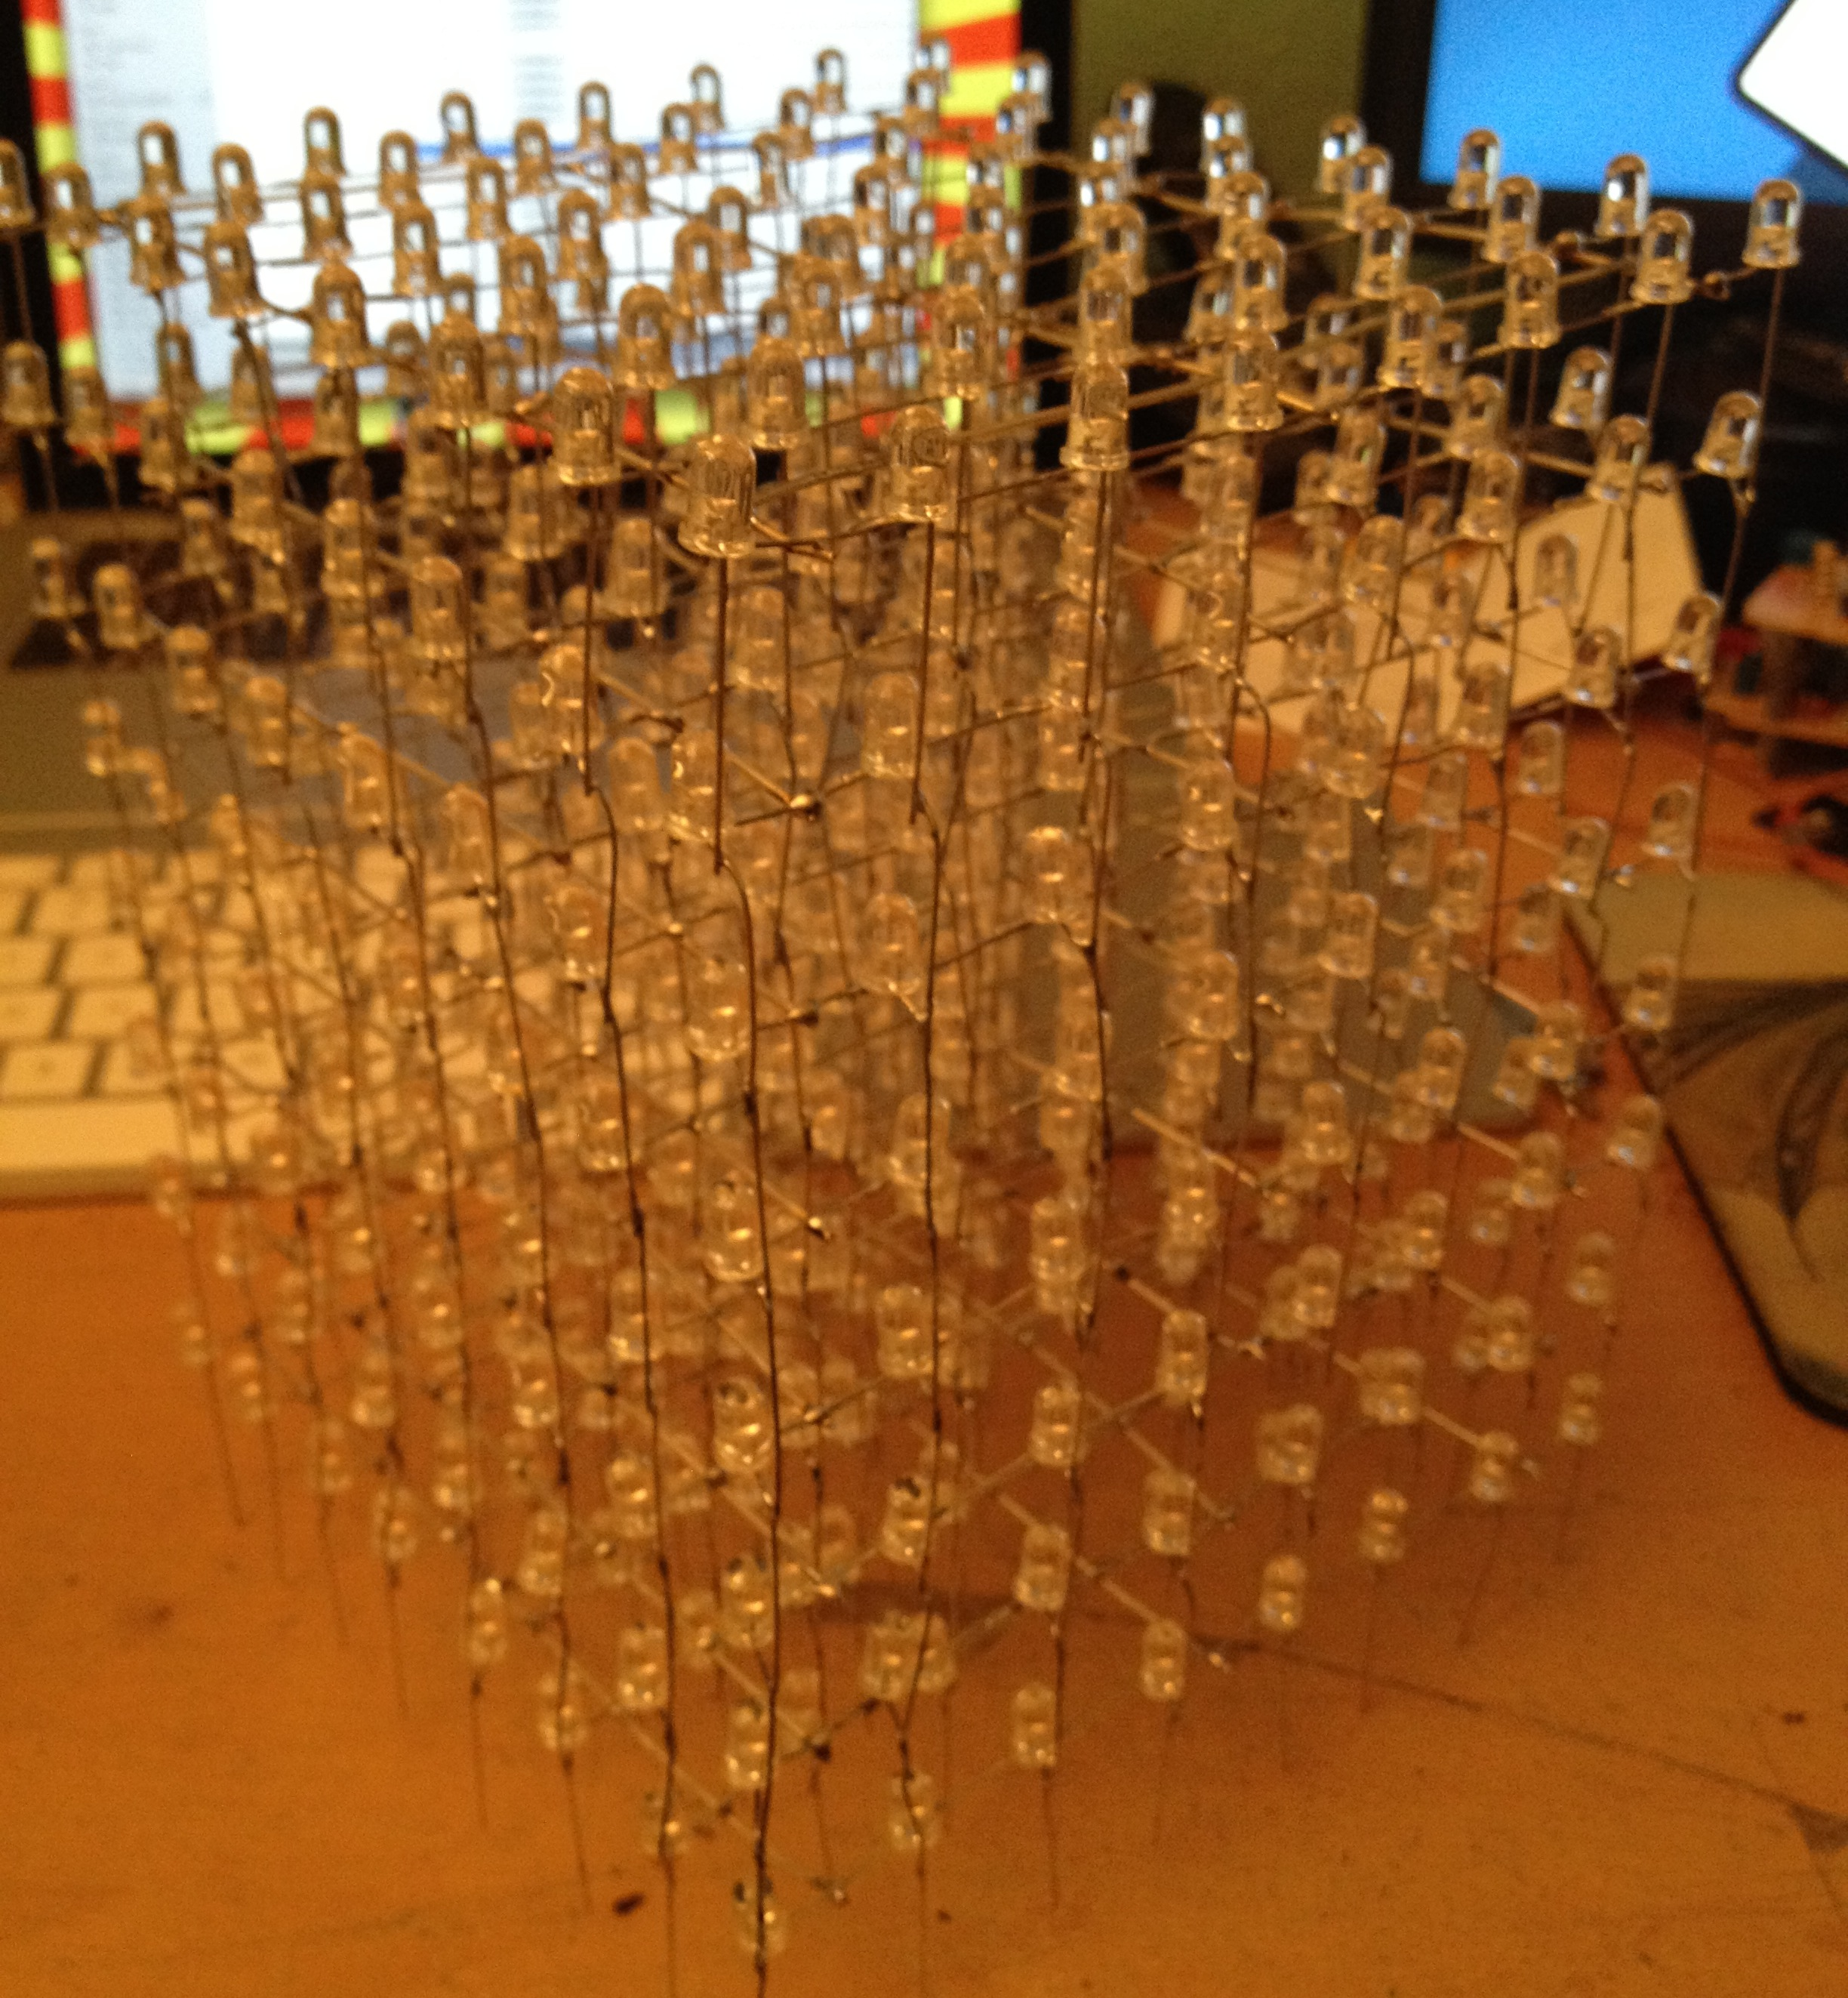
\includegraphics[width=6cm]{cube.jpg}
		\caption{LED Würfel}
		\label{Cube}
	\end{minipage}
	\hfill
	\begin{minipage}[t]{7cm}
		\vspace{0pt}
		Der LED Würfel wird vom AtMega32 mittels Charlieplexing angesteuert. Das heißt, dass jeweils eine Ebene des Würfels, bestehend aus 64 LEDs, angeschaltet ist. So werden alle 8 Ebenen schnell hintereinander angeschaltet, wodurch aufgrund der Trägheit des menschlichen Auges ein ständiges Bild entsteht. Dieser Aufwand ist nötig, um nicht 512 Anschlüsse des Prozessors zu belegen.
	\end{minipage}
\end{figure}

Die Anoden der LEDs sind jeweils bei 8 LEDs einer Säule zusammengelegt, die Kathoden einer ganzen Ebene sind ebenfalls zusammengelegt. Die 64 Anoden werden von 8 8bit Latches angesteuert, die 8 Kathoden werden von N-Kanal Mosfets auf das Massepotential gelegt.
\clearpage

\begin{figure}[hbp]
	\begin{minipage}[t]{7cm}
		\vspace{0pt}
		Der AtMega32 nimmt über den seriellen Port Kommandos und Animationen entgegen. Die Animationen werden in einem per I\textsuperscript{2}C-Bus angeschlossenen F-RAM gespeichert, der auch ohne Spannungsversorgung seine Daten hält. Ausserdem ist über den I\textsuperscript{2}C-Bus der AtMega8 für die Musiksteuerung angeschlossen.
	\end{minipage}
	\hfill
	\begin{minipage}[t]{6cm}
		\vspace{0pt}
		\centering
		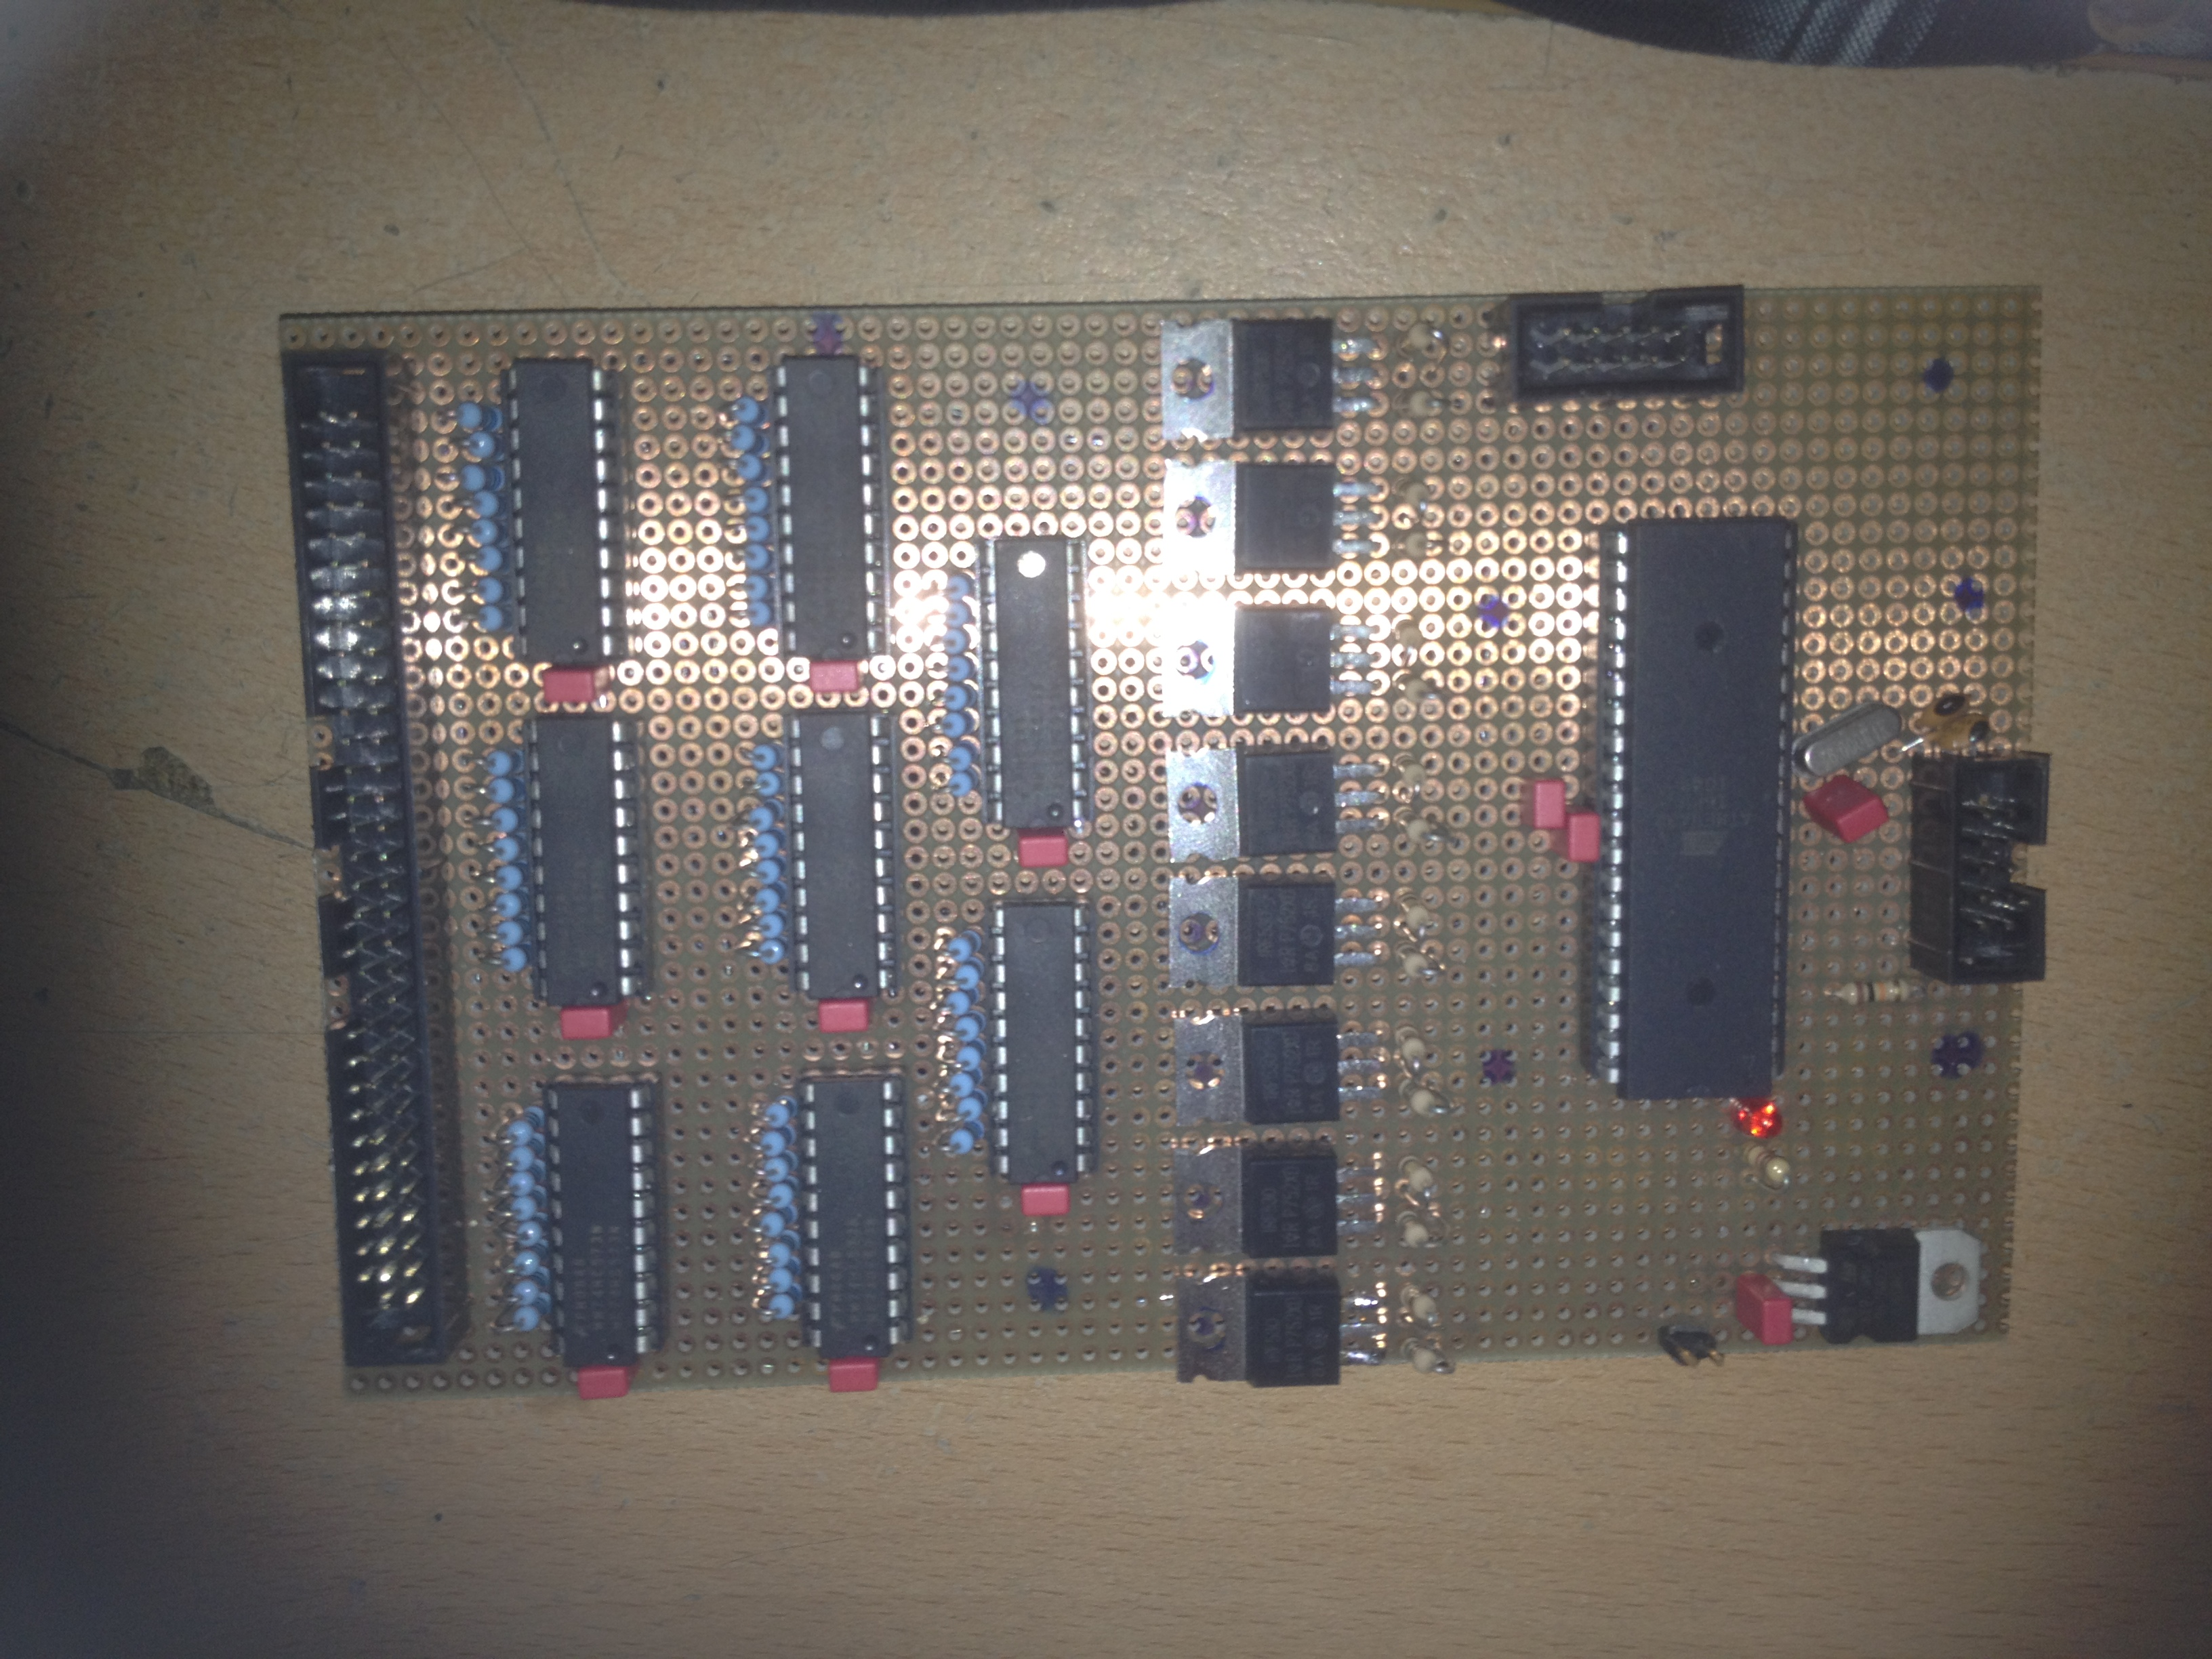
\includegraphics[width=6cm]{platine1.jpg}
		\caption{AtMega32}
		\label{AtMega32}
	\end{minipage}
\end{figure}

% ###############################

\section{Hardware - AtMega8}
\begin{figure}[hbp]
	\begin{minipage}[t]{6cm}
		\vspace{0pt}
		\centering
		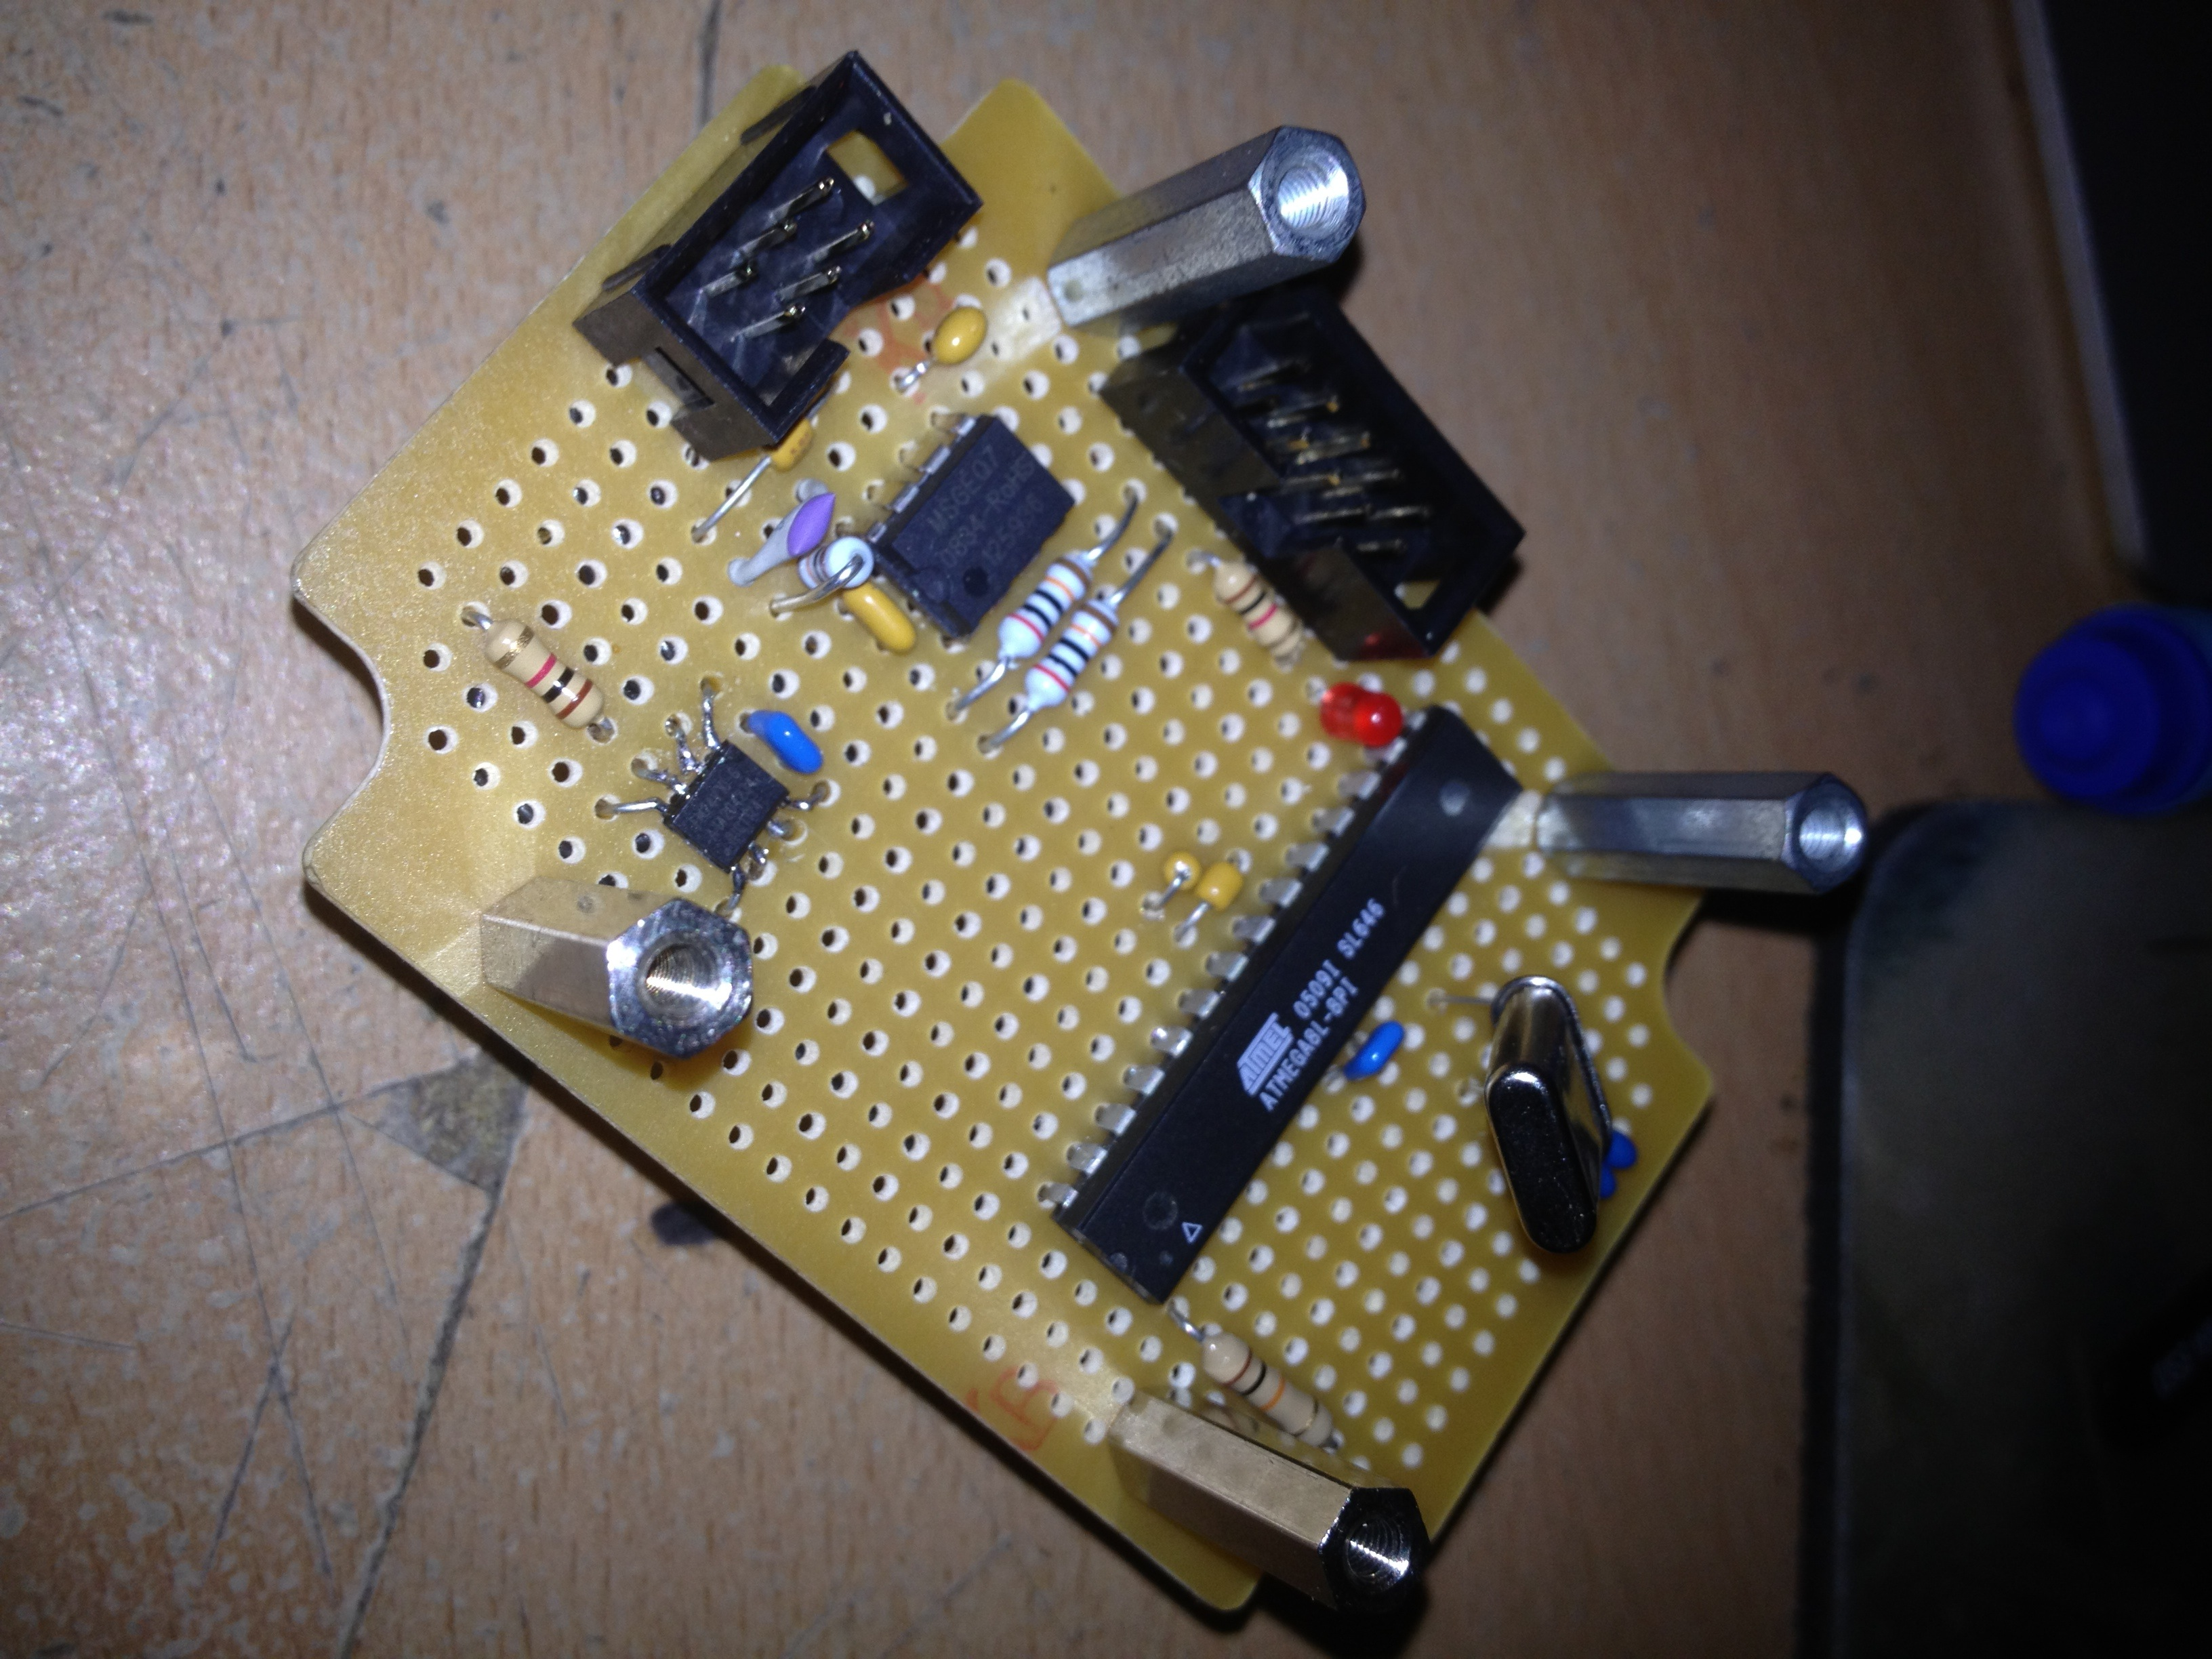
\includegraphics[width=6cm]{platine2.jpg}
		\caption{AtMega8}
		\label{AtMega8}
	\end{minipage}
	\hfill
	\begin{minipage}[t]{7cm}
		\vspace{0pt}
		Der AtMega8 agiert als I\textsuperscript{2}C Slave. Mithilfe eines MSGEQ7, ein \textit{Seven Band Graphic Equalizer}, erhält der AtMega8 die Amplitudenhöhe auf verschiedenen Frequenzbändern eines angeschlossen Audiosignals. Diese Informationen werden, wenn der AtMega32 dies verlangt, über den I\textsuperscript{2}C-Bus gesendet.
	\end{minipage}
\end{figure}
\clearpage
% ###############################

\section{Software}
Die PC-Software zur Erstellung und Übertragung von Animationen für den LED Würfel, genannt \textit{CubeControl}, ist in Java geschrieben. Die serielle Kommunikation wird von einigen C Routinen erledigt. Die Software ist mit Windows und Unixoiden Betriebssystemen kompatibel, Vorraussetzung ist eine Java Runtime Environment und Windows- oder Unix-kompatible Syscalls zur Kommunikation mit seriellen Ports.

\begin{figure}[ht]
	\centering
	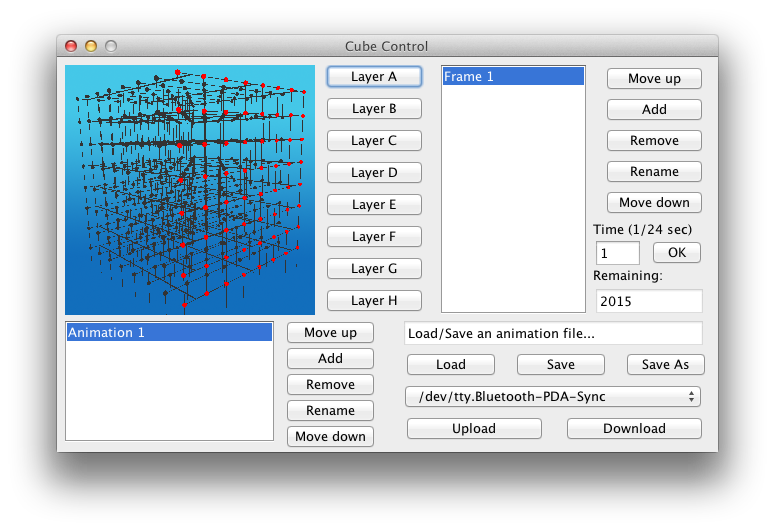
\includegraphics[width=16cm]{CubeControl.png}
	\caption{CubeControl Screenshot}
	\label{CubeControl}
\end{figure}

Eine drehbare, 3 dimensionale Darstellung des LED Würfels in der Software vereinfacht das Erstellen von Animationen.

\end{document}  